% Options for packages loaded elsewhere
\PassOptionsToPackage{unicode}{hyperref}
\PassOptionsToPackage{hyphens}{url}
%
\documentclass[
]{article}
\usepackage{lmodern}
\usepackage{amssymb,amsmath}
\usepackage{ifxetex,ifluatex}
\ifnum 0\ifxetex 1\fi\ifluatex 1\fi=0 % if pdftex
  \usepackage[T1]{fontenc}
  \usepackage[utf8]{inputenc}
  \usepackage{textcomp} % provide euro and other symbols
\else % if luatex or xetex
  \usepackage{unicode-math}
  \defaultfontfeatures{Scale=MatchLowercase}
  \defaultfontfeatures[\rmfamily]{Ligatures=TeX,Scale=1}
\fi
% Use upquote if available, for straight quotes in verbatim environments
\IfFileExists{upquote.sty}{\usepackage{upquote}}{}
\IfFileExists{microtype.sty}{% use microtype if available
  \usepackage[]{microtype}
  \UseMicrotypeSet[protrusion]{basicmath} % disable protrusion for tt fonts
}{}
\makeatletter
\@ifundefined{KOMAClassName}{% if non-KOMA class
  \IfFileExists{parskip.sty}{%
    \usepackage{parskip}
  }{% else
    \setlength{\parindent}{0pt}
    \setlength{\parskip}{6pt plus 2pt minus 1pt}}
}{% if KOMA class
  \KOMAoptions{parskip=half}}
\makeatother
\usepackage{xcolor}
\IfFileExists{xurl.sty}{\usepackage{xurl}}{} % add URL line breaks if available
\IfFileExists{bookmark.sty}{\usepackage{bookmark}}{\usepackage{hyperref}}
\hypersetup{
  pdftitle={02 Data Wrangling Homework},
  pdfauthor={Max Thomasberger},
  hidelinks,
  pdfcreator={LaTeX via pandoc}}
\urlstyle{same} % disable monospaced font for URLs
\usepackage[margin=1in]{geometry}
\usepackage{color}
\usepackage{fancyvrb}
\newcommand{\VerbBar}{|}
\newcommand{\VERB}{\Verb[commandchars=\\\{\}]}
\DefineVerbatimEnvironment{Highlighting}{Verbatim}{commandchars=\\\{\}}
% Add ',fontsize=\small' for more characters per line
\usepackage{framed}
\definecolor{shadecolor}{RGB}{248,248,248}
\newenvironment{Shaded}{\begin{snugshade}}{\end{snugshade}}
\newcommand{\AlertTok}[1]{\textcolor[rgb]{0.94,0.16,0.16}{#1}}
\newcommand{\AnnotationTok}[1]{\textcolor[rgb]{0.56,0.35,0.01}{\textbf{\textit{#1}}}}
\newcommand{\AttributeTok}[1]{\textcolor[rgb]{0.77,0.63,0.00}{#1}}
\newcommand{\BaseNTok}[1]{\textcolor[rgb]{0.00,0.00,0.81}{#1}}
\newcommand{\BuiltInTok}[1]{#1}
\newcommand{\CharTok}[1]{\textcolor[rgb]{0.31,0.60,0.02}{#1}}
\newcommand{\CommentTok}[1]{\textcolor[rgb]{0.56,0.35,0.01}{\textit{#1}}}
\newcommand{\CommentVarTok}[1]{\textcolor[rgb]{0.56,0.35,0.01}{\textbf{\textit{#1}}}}
\newcommand{\ConstantTok}[1]{\textcolor[rgb]{0.00,0.00,0.00}{#1}}
\newcommand{\ControlFlowTok}[1]{\textcolor[rgb]{0.13,0.29,0.53}{\textbf{#1}}}
\newcommand{\DataTypeTok}[1]{\textcolor[rgb]{0.13,0.29,0.53}{#1}}
\newcommand{\DecValTok}[1]{\textcolor[rgb]{0.00,0.00,0.81}{#1}}
\newcommand{\DocumentationTok}[1]{\textcolor[rgb]{0.56,0.35,0.01}{\textbf{\textit{#1}}}}
\newcommand{\ErrorTok}[1]{\textcolor[rgb]{0.64,0.00,0.00}{\textbf{#1}}}
\newcommand{\ExtensionTok}[1]{#1}
\newcommand{\FloatTok}[1]{\textcolor[rgb]{0.00,0.00,0.81}{#1}}
\newcommand{\FunctionTok}[1]{\textcolor[rgb]{0.00,0.00,0.00}{#1}}
\newcommand{\ImportTok}[1]{#1}
\newcommand{\InformationTok}[1]{\textcolor[rgb]{0.56,0.35,0.01}{\textbf{\textit{#1}}}}
\newcommand{\KeywordTok}[1]{\textcolor[rgb]{0.13,0.29,0.53}{\textbf{#1}}}
\newcommand{\NormalTok}[1]{#1}
\newcommand{\OperatorTok}[1]{\textcolor[rgb]{0.81,0.36,0.00}{\textbf{#1}}}
\newcommand{\OtherTok}[1]{\textcolor[rgb]{0.56,0.35,0.01}{#1}}
\newcommand{\PreprocessorTok}[1]{\textcolor[rgb]{0.56,0.35,0.01}{\textit{#1}}}
\newcommand{\RegionMarkerTok}[1]{#1}
\newcommand{\SpecialCharTok}[1]{\textcolor[rgb]{0.00,0.00,0.00}{#1}}
\newcommand{\SpecialStringTok}[1]{\textcolor[rgb]{0.31,0.60,0.02}{#1}}
\newcommand{\StringTok}[1]{\textcolor[rgb]{0.31,0.60,0.02}{#1}}
\newcommand{\VariableTok}[1]{\textcolor[rgb]{0.00,0.00,0.00}{#1}}
\newcommand{\VerbatimStringTok}[1]{\textcolor[rgb]{0.31,0.60,0.02}{#1}}
\newcommand{\WarningTok}[1]{\textcolor[rgb]{0.56,0.35,0.01}{\textbf{\textit{#1}}}}
\usepackage{graphicx,grffile}
\makeatletter
\def\maxwidth{\ifdim\Gin@nat@width>\linewidth\linewidth\else\Gin@nat@width\fi}
\def\maxheight{\ifdim\Gin@nat@height>\textheight\textheight\else\Gin@nat@height\fi}
\makeatother
% Scale images if necessary, so that they will not overflow the page
% margins by default, and it is still possible to overwrite the defaults
% using explicit options in \includegraphics[width, height, ...]{}
\setkeys{Gin}{width=\maxwidth,height=\maxheight,keepaspectratio}
% Set default figure placement to htbp
\makeatletter
\def\fps@figure{htbp}
\makeatother
\setlength{\emergencystretch}{3em} % prevent overfull lines
\providecommand{\tightlist}{%
  \setlength{\itemsep}{0pt}\setlength{\parskip}{0pt}}
\setcounter{secnumdepth}{-\maxdimen} % remove section numbering
\usepackage{booktabs}
\usepackage{longtable}
\usepackage{array}
\usepackage{multirow}
\usepackage{wrapfig}
\usepackage{float}
\usepackage{colortbl}
\usepackage{pdflscape}
\usepackage{tabu}
\usepackage{threeparttable}
\usepackage{threeparttablex}
\usepackage[normalem]{ulem}
\usepackage{makecell}
\usepackage{xcolor}

\title{02 Data Wrangling Homework}
\usepackage{etoolbox}
\makeatletter
\providecommand{\subtitle}[1]{% add subtitle to \maketitle
  \apptocmd{\@title}{\par {\large #1 \par}}{}{}
}
\makeatother
\subtitle{Data Science and Machine Learning 2187 \& 2087}
\author{Max Thomasberger}
\date{11 2020}

\begin{document}
\maketitle

{
\setcounter{tocdepth}{2}
\tableofcontents
}
\hypertarget{please-enter-details-about-your-group-here}{%
\section{PLEASE ENTER DETAILS ABOUT YOUR GROUP
HERE}\label{please-enter-details-about-your-group-here}}

\begin{quote}
\textbf{GROUP 4}
\end{quote}

\textbf{Leonard Fidlin}, h01352705

\textbf{Daniel Jost}, h01451889

\textbf{Anne Valder}, h11928415

\hypertarget{introduction}{%
\section{Introduction}\label{introduction}}

Note: this Rmarkdown file downloads a 78 MB zip file from a server when
you knit it.

Please limit your outputs to the first few results using the
\textbf{head()} function after filtering or re-arranging the data. If I
recieve HTML files containing endless lists of names the respective
group will get \(l o O o 0 s e\) points!

Here's how you should do it:

\begin{Shaded}
\begin{Highlighting}[]
\CommentTok{# This only shows the first few rows of the data frame after knitting}

\NormalTok{babynames }\OperatorTok
\StringTok{  }\KeywordTok{head}\NormalTok{()}
\end{Highlighting}
\end{Shaded}

\begin{verbatim}
##   year sex      name    n       prop
## 1 1880   F      Mary 7065 0.07238359
## 2 1880   F      Anna 2604 0.02667896
## 3 1880   F      Emma 2003 0.02052149
## 4 1880   F Elizabeth 1939 0.01986579
## 5 1880   F    Minnie 1746 0.01788843
## 6 1880   F  Margaret 1578 0.01616720
\end{verbatim}

18 points are possible for this homework. Each code chunk you enter is
worth 1 point. The real world example is in total worth 6 points and a
bit tricky but I am inclined to be generous if you at least try it.

The homework is due on Thursday 03-12-2020 at 23:59. Please upload your
answers as HTML file to \href{mailto:learn@WU}{\nolinkurl{learn@WU}}. I
will draw a random course participant on the Friday 04-12-2020 lecture
to walk us through some of the exercises.

\hypertarget{select}{%
\section{Select}\label{select}}

Alter the code below to select just the \texttt{prop} column:

\begin{Shaded}
\begin{Highlighting}[]
\KeywordTok{select}\NormalTok{(babynames, prop) }\OperatorTok
\StringTok{  }\KeywordTok{head}\NormalTok{()}
\end{Highlighting}
\end{Shaded}

\begin{verbatim}
##         prop
## 1 0.07238359
## 2 0.02667896
## 3 0.02052149
## 4 0.01986579
## 5 0.01788843
## 6 0.01616720
\end{verbatim}

\hypertarget{filter-1}{%
\section{Filter 1}\label{filter-1}}

Show:

\begin{itemize}
\tightlist
\item
  All names where prop is greater than or equal to 0.05 and smaller than
  0.8
\item
  All children named ``Max'' and ``Moritz''
\item
  All of the rows that have a missing value for \texttt{name}.
\end{itemize}

\textbf{Only display the first few results using the head() function.}

\begin{Shaded}
\begin{Highlighting}[]
\KeywordTok{filter}\NormalTok{(babynames, }\FloatTok{0.05}\OperatorTok{<=}\NormalTok{prop, prop}\OperatorTok{<=}\FloatTok{0.80}\NormalTok{)  }\OperatorTok\StringTok{ }
\StringTok{  }\KeywordTok{head}\NormalTok{()}
\end{Highlighting}
\end{Shaded}

\begin{verbatim}
##   year sex    name    n       prop
## 1 1880   F    Mary 7065 0.07238359
## 2 1880   M    John 9655 0.08154561
## 3 1880   M William 9532 0.08050676
## 4 1880   M   James 5927 0.05005912
## 5 1881   F    Mary 6919 0.06999140
## 6 1881   M    John 8769 0.08098299
\end{verbatim}

\begin{Shaded}
\begin{Highlighting}[]
\KeywordTok{filter}\NormalTok{(babynames, name }\OperatorTok\StringTok{ }\KeywordTok{c}\NormalTok{(}\StringTok{"Max"}\NormalTok{,}\StringTok{"Moritz"}\NormalTok{))  }\OperatorTok\StringTok{ }
\StringTok{  }\KeywordTok{head}\NormalTok{()}
\end{Highlighting}
\end{Shaded}

\begin{verbatim}
##   year sex name  n       prop
## 1 1880   M  Max 52 0.00043919
## 2 1881   M  Max 66 0.00060952
## 3 1882   M  Max 74 0.00060640
## 4 1883   M  Max 75 0.00066680
## 5 1884   M  Max 80 0.00065179
## 6 1885   M  Max 71 0.00061236
\end{verbatim}

\begin{Shaded}
\begin{Highlighting}[]
\KeywordTok{filter}\NormalTok{(babynames, }\KeywordTok{is.na}\NormalTok{(name))  }\OperatorTok\StringTok{ }
\StringTok{  }\KeywordTok{head}\NormalTok{()}
\end{Highlighting}
\end{Shaded}

\begin{verbatim}
## [1] year sex  name n    prop
## <0 rows> (or 0-length row.names)
\end{verbatim}

\hypertarget{filter-2}{%
\section{Filter 2}\label{filter-2}}

Use Boolean operators to return only the rows of the babyname object
that contain:

\begin{itemize}
\tightlist
\item
  Girls named Max
\item
  Names that were used by exactly 5 or 6 children in 1990
\item
  Names that are one of Max, Moritz, or Wilhelm
\end{itemize}

\textbf{Only display the first few results using the head() function.}

\begin{Shaded}
\begin{Highlighting}[]
\KeywordTok{filter}\NormalTok{(babynames, sex}\OperatorTok{==}\StringTok{"F"} \OperatorTok{&}\StringTok{ }\NormalTok{name}\OperatorTok{==}\StringTok{"Max"}\NormalTok{) }\OperatorTok\StringTok{ }
\StringTok{  }\KeywordTok{head}\NormalTok{()}
\end{Highlighting}
\end{Shaded}

\begin{verbatim}
##   year sex name  n     prop
## 1 1912   F  Max  5 8.52e-06
## 2 1914   F  Max  6 7.53e-06
## 3 1917   F  Max  7 6.23e-06
## 4 1918   F  Max  8 6.65e-06
## 5 1919   F  Max 11 9.36e-06
## 6 1920   F  Max 10 8.04e-06
\end{verbatim}

\begin{Shaded}
\begin{Highlighting}[]
\NormalTok{babynames }\OperatorTok\StringTok{ }\KeywordTok{filter}\NormalTok{(year }\OperatorTok{==}\StringTok{ }\DecValTok{1990} \OperatorTok{&}\StringTok{ }\NormalTok{(n}\OperatorTok{==}\DecValTok{5}\OperatorTok{|}\NormalTok{n}\OperatorTok{==}\DecValTok{6}\NormalTok{)) }\OperatorTok\StringTok{ }
\StringTok{  }\KeywordTok{head}\NormalTok{()}
\end{Highlighting}
\end{Shaded}

\begin{verbatim}
##   year sex     name n     prop
## 1 1990   F   Aariel 6 2.92e-06
## 2 1990   F   Aarion 6 2.92e-06
## 3 1990   F  Abagael 6 2.92e-06
## 4 1990   F    Abbye 6 2.92e-06
## 5 1990   F   Abiola 6 2.92e-06
## 6 1990   F Abreanna 6 2.92e-06
\end{verbatim}

\begin{Shaded}
\begin{Highlighting}[]
\KeywordTok{filter}\NormalTok{(babynames, name}\OperatorTok{==}\StringTok{"Max"} \OperatorTok{|}\StringTok{ }\NormalTok{name}\OperatorTok{==}\StringTok{"Moritz"} \OperatorTok{|}\StringTok{ }\NormalTok{name}\OperatorTok{==}\StringTok{"Wilhelm"}\NormalTok{) }\OperatorTok\StringTok{ }
\StringTok{  }\KeywordTok{head}\NormalTok{()}
\end{Highlighting}
\end{Shaded}

\begin{verbatim}
##   year sex    name  n       prop
## 1 1880   M     Max 52 0.00043919
## 2 1880   M Wilhelm  6 0.00005068
## 3 1881   M     Max 66 0.00060952
## 4 1882   M     Max 74 0.00060640
## 5 1882   M Wilhelm  6 0.00004917
## 6 1883   M     Max 75 0.00066680
\end{verbatim}

\hypertarget{arrange}{%
\section{Arrange}\label{arrange}}

Arrange babynames by \texttt{n}. Add \texttt{prop} as a second (tie
breaking) variable to arrange on. Can you tell what the smallest value
of \texttt{n} is?

\textbf{Only display the first few results using the head() function.}

\begin{Shaded}
\begin{Highlighting}[]
\KeywordTok{arrange}\NormalTok{(babynames, n, prop) }\OperatorTok\StringTok{ }
\StringTok{  }\KeywordTok{head}\NormalTok{()}
\end{Highlighting}
\end{Shaded}

\begin{verbatim}
##   year sex       name n     prop
## 1 2007   M      Aaban 5 2.26e-06
## 2 2007   M     Aareon 5 2.26e-06
## 3 2007   M      Aaris 5 2.26e-06
## 4 2007   M        Abd 5 2.26e-06
## 5 2007   M Abdulazeez 5 2.26e-06
## 6 2007   M  Abdulhadi 5 2.26e-06
\end{verbatim}

\begin{Shaded}
\begin{Highlighting}[]
\KeywordTok{min}\NormalTok{(babynames}\OperatorTok{$}\NormalTok{n)}
\end{Highlighting}
\end{Shaded}

\begin{verbatim}
## [1] 5
\end{verbatim}

The smallest value of \texttt{n} is 5.

\hypertarget{desc}{%
\section{Desc}\label{desc}}

Use \texttt{desc()} to find the names with the highest prop.

Then, use \texttt{desc()} to find the names with the highest n.

\textbf{Only display the first few results using the head() function.}

\begin{Shaded}
\begin{Highlighting}[]
\KeywordTok{arrange}\NormalTok{(babynames, }\KeywordTok{desc}\NormalTok{(prop)) }\OperatorTok\StringTok{ }
\StringTok{  }\KeywordTok{head}\NormalTok{()}
\end{Highlighting}
\end{Shaded}

\begin{verbatim}
##   year sex    name    n       prop
## 1 1880   M    John 9655 0.08154561
## 2 1881   M    John 8769 0.08098299
## 3 1880   M William 9532 0.08050676
## 4 1883   M    John 8894 0.07907394
## 5 1881   M William 8524 0.07872038
## 6 1882   M    John 9557 0.07831617
\end{verbatim}

\begin{Shaded}
\begin{Highlighting}[]
\KeywordTok{arrange}\NormalTok{(babynames, }\KeywordTok{desc}\NormalTok{(n)) }\OperatorTok\StringTok{ }
\StringTok{  }\KeywordTok{head}\NormalTok{()}
\end{Highlighting}
\end{Shaded}

\begin{verbatim}
##   year sex    name     n       prop
## 1 1947   F   Linda 99686 0.05483812
## 2 1948   F   Linda 96209 0.05521079
## 3 1947   M   James 94756 0.05101589
## 4 1957   M Michael 92695 0.04237565
## 5 1947   M  Robert 91642 0.04933934
## 6 1949   F   Linda 91016 0.05184643
\end{verbatim}

\hypertarget{steps-and-the-pipe}{%
\section{Steps and the pipe}\label{steps-and-the-pipe}}

Use \texttt{\%\textgreater{}\%} to write a sequence of functions that:

\begin{enumerate}
\def\labelenumi{\arabic{enumi}.}
\tightlist
\item
  Filter babynames to just the boys that were born in 1990\\
\item
  Select the \texttt{prop} and \texttt{name} columns\\
\item
  Arrange the results so that the most popular names are near the top.
\item
  Only show the first few results using the head() function
\end{enumerate}

\begin{Shaded}
\begin{Highlighting}[]
\NormalTok{babynames }\OperatorTok\StringTok{ }
\KeywordTok{filter}\NormalTok{(sex}\OperatorTok{==}\StringTok{"M"}\NormalTok{, year}\OperatorTok{==}\DecValTok{1990}\NormalTok{) }\OperatorTok\StringTok{ }
\StringTok{  }\KeywordTok{select}\NormalTok{(prop, name) }\OperatorTok\StringTok{ }
\StringTok{  }\KeywordTok{arrange}\NormalTok{(}\KeywordTok{desc}\NormalTok{(prop)) }\OperatorTok\StringTok{ }
\StringTok{  }\KeywordTok{head}\NormalTok{()}
\end{Highlighting}
\end{Shaded}

\begin{verbatim}
##         prop        name
## 1 0.03034735     Michael
## 2 0.02432734 Christopher
## 3 0.02082597     Matthew
## 4 0.02008963      Joshua
## 5 0.01571943      Daniel
## 6 0.01568549       David
\end{verbatim}

\hypertarget{steps-and-the-pipe-1}{%
\section{Steps and the pipe}\label{steps-and-the-pipe-1}}

Chain the following steps together using the pipe
\texttt{\%\textgreater{}\%} operator.

\begin{enumerate}
\def\labelenumi{\arabic{enumi}.}
\tightlist
\item
  Trim \texttt{babynames} to just the rows that contain one of your
  \texttt{name}s and your \texttt{sex} (if your name is not in there use
  the name and sex of your favorite movie star)
\item
  Using ggplot2 plot the results as a line graph with \texttt{year} on
  the x axis and \texttt{prop} on the y axis
\end{enumerate}

\begin{Shaded}
\begin{Highlighting}[]
\NormalTok{dan <-}\StringTok{ }\NormalTok{babynames }\OperatorTok\StringTok{ }
\StringTok{  }\KeywordTok{filter}\NormalTok{(name}\OperatorTok{==}\StringTok{"Daniel"}\NormalTok{, sex}\OperatorTok{==}\StringTok{"M"}\NormalTok{)}

\KeywordTok{ggplot}\NormalTok{(dan, }\KeywordTok{aes}\NormalTok{(year, prop)) }\OperatorTok{+}
\StringTok{  }\KeywordTok{geom_line}\NormalTok{()}
\end{Highlighting}
\end{Shaded}

\begin{center}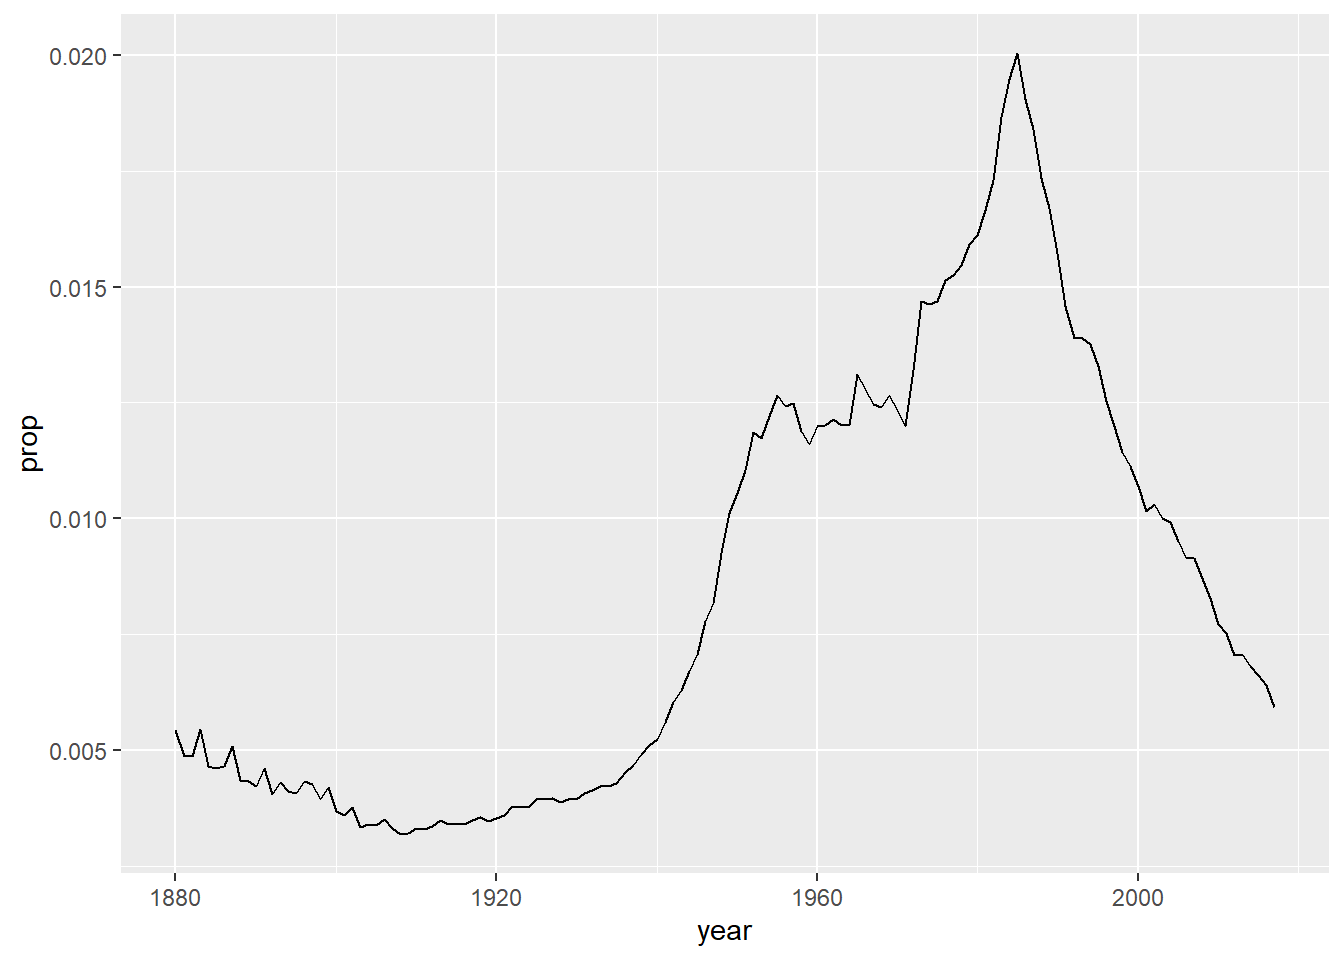
\includegraphics{02_Data_wrangling_homework_files/figure-latex/unnamed-chunk-8-1} \end{center}

Or all our names in one plot:

\begin{Shaded}
\begin{Highlighting}[]
\NormalTok{leo <-}\StringTok{ }\NormalTok{babynames }\OperatorTok\StringTok{ }
\StringTok{  }\KeywordTok{filter}\NormalTok{(name}\OperatorTok{==}\StringTok{"Leonard"}\NormalTok{, sex}\OperatorTok{==}\StringTok{"M"}\NormalTok{)}

\NormalTok{ann <-}\StringTok{ }\NormalTok{babynames }\OperatorTok\StringTok{ }
\StringTok{  }\KeywordTok{filter}\NormalTok{(name}\OperatorTok{==}\StringTok{"Anne"}\NormalTok{, sex}\OperatorTok{==}\StringTok{"F"}\NormalTok{)}

\NormalTok{all <-}\StringTok{ }\KeywordTok{union}\NormalTok{(dan, leo, }\DataTypeTok{id=}\StringTok{"year"}\NormalTok{)}
\NormalTok{all <-}\StringTok{ }\KeywordTok{union}\NormalTok{(all, ann, }\DataTypeTok{id=}\StringTok{"year"}\NormalTok{)}
  
\KeywordTok{ggplot}\NormalTok{(all) }\OperatorTok{+}
\StringTok{  }\KeywordTok{geom_line}\NormalTok{(}\KeywordTok{aes}\NormalTok{(year, prop, }\DataTypeTok{group =}\NormalTok{ name, }\DataTypeTok{color =}\NormalTok{ name))}
\end{Highlighting}
\end{Shaded}

\begin{center}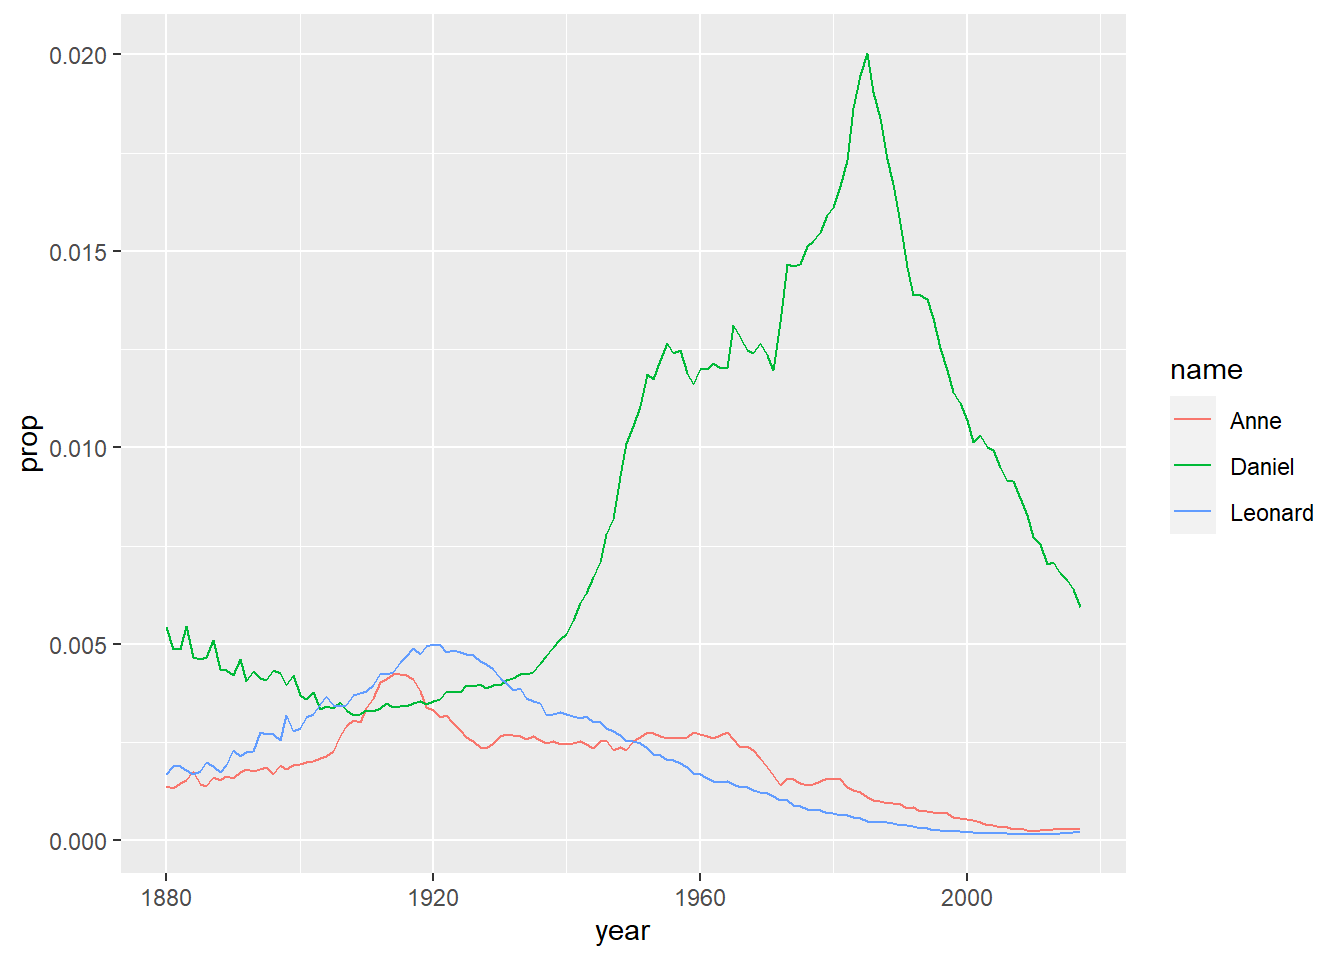
\includegraphics{02_Data_wrangling_homework_files/figure-latex/unnamed-chunk-9-1} \end{center}

\hypertarget{summarise}{%
\section{Summarise}\label{summarise}}

Here some code to remind you how summarise works:

\begin{Shaded}
\begin{Highlighting}[]
\NormalTok{pollution }\OperatorTok\StringTok{ }
\StringTok{ }\KeywordTok{summarise}\NormalTok{(}\DataTypeTok{mean =} \KeywordTok{mean}\NormalTok{(amount), }\DataTypeTok{sum =} \KeywordTok{sum}\NormalTok{(amount), }\DataTypeTok{n =} \KeywordTok{n}\NormalTok{())}
\end{Highlighting}
\end{Shaded}

\begin{verbatim}
## # A tibble: 1 x 3
##    mean   sum     n
##   <dbl> <dbl> <int>
## 1    42   252     6
\end{verbatim}

Now use summarise() to compute three statistics about the babynames
data:

\begin{enumerate}
\def\labelenumi{\arabic{enumi}.}
\tightlist
\item
  The first (minimum) year in the dataset\\
\item
  The last (maximum) year in the dataset\\
\item
  The total number of children represented in the data
\end{enumerate}

\begin{Shaded}
\begin{Highlighting}[]
\NormalTok{babynames }\OperatorTok\StringTok{ }
\StringTok{  }\KeywordTok{summarise}\NormalTok{(}\KeywordTok{min}\NormalTok{(year), }\KeywordTok{max}\NormalTok{(year), }\DataTypeTok{sum =} \KeywordTok{sum}\NormalTok{(n))  }\OperatorTok\StringTok{ }
\StringTok{  }\KeywordTok{head}\NormalTok{()}
\end{Highlighting}
\end{Shaded}

\begin{verbatim}
##   min(year) max(year)       sum
## 1      1880      2017 348120517
\end{verbatim}

\hypertarget{filtering-and-wrangling}{%
\section{Filtering and wrangling}\label{filtering-and-wrangling}}

Extract the rows where \texttt{name\ ==\ "Khaleesi"}. Then use
\texttt{summarise()} and a summary functions to find:

\begin{enumerate}
\def\labelenumi{\arabic{enumi}.}
\tightlist
\item
  The total number of children named Khaleesi
\item
  The first year Khaleesi appeared in the data
\end{enumerate}

\begin{Shaded}
\begin{Highlighting}[]
\NormalTok{babynames }\OperatorTok\StringTok{ }
\KeywordTok{filter}\NormalTok{(name }\OperatorTok{==}\StringTok{ "Khaleesi"}\NormalTok{) }\OperatorTok
\StringTok{  }\KeywordTok{summarise}\NormalTok{(}\DataTypeTok{sum =} \KeywordTok{sum}\NormalTok{(n), }\KeywordTok{min}\NormalTok{(year))  }\OperatorTok\StringTok{ }
\StringTok{  }\KeywordTok{head}\NormalTok{()}
\end{Highlighting}
\end{Shaded}

\begin{verbatim}
##    sum min(year)
## 1 1964      2011
\end{verbatim}

\begin{enumerate}
\def\labelenumi{\arabic{enumi}.}
\tightlist
\item
  1964 is the total number of children named Khaleesi in the sample
\item
  2011 is the first year Khaleesi appeared in the data
\end{enumerate}

\hypertarget{split-apply-combine}{%
\section{Split apply combine}\label{split-apply-combine}}

Here some code to remind you how \texttt{group\_by()} and
\texttt{summarise()} work:

\begin{Shaded}
\begin{Highlighting}[]
\NormalTok{pollution }\OperatorTok\StringTok{ }
\StringTok{  }\KeywordTok{group_by}\NormalTok{(city) }\OperatorTok
\StringTok{  }\KeywordTok{summarise}\NormalTok{(}\DataTypeTok{mean =} \KeywordTok{mean}\NormalTok{(amount), }\DataTypeTok{sum =} \KeywordTok{sum}\NormalTok{(amount), }\DataTypeTok{n =} \KeywordTok{n}\NormalTok{())}
\end{Highlighting}
\end{Shaded}

\begin{verbatim}
## `summarise()` ungrouping output (override with `.groups` argument)
\end{verbatim}

\begin{verbatim}
## # A tibble: 3 x 4
##   city      mean   sum     n
##   <chr>    <dbl> <dbl> <int>
## 1 Beijing   88.5   177     2
## 2 London    19      38     2
## 3 New York  18.5    37     2
\end{verbatim}

Now use \texttt{group\_by()}, \texttt{summarise()}, and
\texttt{arrange()} to display the ten most popular baby names using the
\texttt{head(10)} command. Compute popularity as the total number of
children of a single gender given a name.

\begin{Shaded}
\begin{Highlighting}[]
\NormalTok{babynames }\OperatorTok\StringTok{ }
\KeywordTok{group_by}\NormalTok{(sex, name) }\OperatorTok\StringTok{ }
\KeywordTok{summarise}\NormalTok{(}\DataTypeTok{sum =} \KeywordTok{sum}\NormalTok{(n)) }\OperatorTok\StringTok{ }
\KeywordTok{arrange}\NormalTok{(}\KeywordTok{desc}\NormalTok{(sum)) }\OperatorTok\StringTok{ }
\KeywordTok{head}\NormalTok{(}\DecValTok{10}\NormalTok{)}
\end{Highlighting}
\end{Shaded}

\begin{verbatim}
## `summarise()` regrouping output by 'sex' (override with `.groups` argument)
\end{verbatim}

\begin{verbatim}
## # A tibble: 10 x 3
## # Groups:   sex [2]
##    sex   name        sum
##    <chr> <chr>     <int>
##  1 M     James   5150472
##  2 M     John    5115466
##  3 M     Robert  4814815
##  4 M     Michael 4350824
##  5 F     Mary    4123200
##  6 M     William 4102604
##  7 M     David   3611329
##  8 M     Joseph  2603445
##  9 M     Richard 2563082
## 10 M     Charles 2386048
\end{verbatim}

\hypertarget{mutate}{%
\section{Mutate}\label{mutate}}

Here some code to remind you how \texttt{mutate()} works:

\begin{Shaded}
\begin{Highlighting}[]
\NormalTok{babynames }\OperatorTok
\StringTok{  }\KeywordTok{mutate}\NormalTok{(}\DataTypeTok{percent =} \KeywordTok{round}\NormalTok{(prop}\OperatorTok{*}\DecValTok{100}\NormalTok{, }\DecValTok{2}\NormalTok{)) }\OperatorTok
\StringTok{  }\KeywordTok{head}\NormalTok{()}
\end{Highlighting}
\end{Shaded}

\begin{verbatim}
##   year sex      name    n       prop percent
## 1 1880   F      Mary 7065 0.07238359    7.24
## 2 1880   F      Anna 2604 0.02667896    2.67
## 3 1880   F      Emma 2003 0.02052149    2.05
## 4 1880   F Elizabeth 1939 0.01986579    1.99
## 5 1880   F    Minnie 1746 0.01788843    1.79
## 6 1880   F  Margaret 1578 0.01616720    1.62
\end{verbatim}

Now use \texttt{min\_rank()} and \texttt{mutate()} to rank each row in
\texttt{babynames} from largest \texttt{n} to smallest \texttt{n}.

\textbf{Only display the first few results using the head() function.}

\begin{Shaded}
\begin{Highlighting}[]
\NormalTok{babynames }\OperatorTok\StringTok{ }
\StringTok{  }\KeywordTok{mutate}\NormalTok{(}\DataTypeTok{rank =} \KeywordTok{min_rank}\NormalTok{(}\KeywordTok{desc}\NormalTok{(n))) }\OperatorTok\StringTok{ }
\StringTok{  }\KeywordTok{arrange}\NormalTok{(rank) }\OperatorTok\StringTok{ }
\StringTok{  }\KeywordTok{head}\NormalTok{()}
\end{Highlighting}
\end{Shaded}

\begin{verbatim}
##   year sex    name     n       prop rank
## 1 1947   F   Linda 99686 0.05483812    1
## 2 1948   F   Linda 96209 0.05521079    2
## 3 1947   M   James 94756 0.05101589    3
## 4 1957   M Michael 92695 0.04237565    4
## 5 1947   M  Robert 91642 0.04933934    5
## 6 1949   F   Linda 91016 0.05184643    6
\end{verbatim}

Compute each name's rank \emph{within its year and sex}. Then compute
the median rank \emph{for each combination of name and sex}, and arrange
the results from highest median rank to lowest.

\begin{Shaded}
\begin{Highlighting}[]
\NormalTok{babynames }\OperatorTok\StringTok{ }
\StringTok{  }\KeywordTok{group_by}\NormalTok{(year, sex) }\OperatorTok\StringTok{ }
\StringTok{  }\KeywordTok{group_by}\NormalTok{(name, sex) }\OperatorTok\StringTok{ }
\StringTok{  }\KeywordTok{mutate}\NormalTok{(}\DataTypeTok{rank_ys =} \KeywordTok{min_rank}\NormalTok{(}\KeywordTok{desc}\NormalTok{(n))) }\OperatorTok\StringTok{ }
\StringTok{  }\KeywordTok{mutate}\NormalTok{(}\DataTypeTok{med_rank_ys =} \KeywordTok{median}\NormalTok{(rank_ys)) }\OperatorTok\StringTok{ }
\StringTok{  }\KeywordTok{arrange}\NormalTok{(}\KeywordTok{desc}\NormalTok{(med_rank_ys)) }\OperatorTok\StringTok{ }
\StringTok{  }\KeywordTok{head}\NormalTok{()}
\end{Highlighting}
\end{Shaded}

\begin{verbatim}
## # A tibble: 6 x 7
## # Groups:   name, sex [6]
##    year sex   name          n   prop rank_ys med_rank_ys
##   <dbl> <chr> <chr>     <int>  <dbl>   <int>       <dbl>
## 1  1880 F     Mary       7065 0.0724     115        69.5
## 2  1880 F     Anna       2604 0.0267     138        69.5
## 3  1880 F     Emma       2003 0.0205      97        69.5
## 4  1880 F     Elizabeth  1939 0.0199     137        69.5
## 5  1880 F     Minnie     1746 0.0179      52        69.5
## 6  1880 F     Margaret   1578 0.0162     138        69.5
\end{verbatim}

\hypertarget{joining-data}{%
\section{Joining data}\label{joining-data}}

Here some code to remind you of the types of joins we looked at in
class:

\begin{Shaded}
\begin{Highlighting}[]
\NormalTok{band }\OperatorTok\StringTok{ }\KeywordTok{left_join}\NormalTok{(instrument, }\DataTypeTok{by =} \StringTok{"name"}\NormalTok{)}
\end{Highlighting}
\end{Shaded}

\begin{verbatim}
## # A tibble: 3 x 3
##   name  band    plays 
##   <chr> <chr>   <chr> 
## 1 Mick  Stones  <NA>  
## 2 John  Beatles guitar
## 3 Paul  Beatles bass
\end{verbatim}

\begin{Shaded}
\begin{Highlighting}[]
\NormalTok{band }\OperatorTok\StringTok{ }\KeywordTok{right_join}\NormalTok{(instrument, }\DataTypeTok{by =} \StringTok{"name"}\NormalTok{)}
\end{Highlighting}
\end{Shaded}

\begin{verbatim}
## # A tibble: 3 x 3
##   name  band    plays 
##   <chr> <chr>   <chr> 
## 1 John  Beatles guitar
## 2 Paul  Beatles bass  
## 3 Keith <NA>    guitar
\end{verbatim}

\begin{Shaded}
\begin{Highlighting}[]
\NormalTok{band }\OperatorTok\StringTok{ }\KeywordTok{full_join}\NormalTok{(instrument, }\DataTypeTok{by =} \StringTok{"name"}\NormalTok{)}
\end{Highlighting}
\end{Shaded}

\begin{verbatim}
## # A tibble: 4 x 3
##   name  band    plays 
##   <chr> <chr>   <chr> 
## 1 Mick  Stones  <NA>  
## 2 John  Beatles guitar
## 3 Paul  Beatles bass  
## 4 Keith <NA>    guitar
\end{verbatim}

\begin{Shaded}
\begin{Highlighting}[]
\NormalTok{band }\OperatorTok\StringTok{ }\KeywordTok{inner_join}\NormalTok{(instrument, }\DataTypeTok{by =} \StringTok{"name"}\NormalTok{)}
\end{Highlighting}
\end{Shaded}

\begin{verbatim}
## # A tibble: 2 x 3
##   name  band    plays 
##   <chr> <chr>   <chr> 
## 1 John  Beatles guitar
## 2 Paul  Beatles bass
\end{verbatim}

\hypertarget{left-join}{%
\section{Left join}\label{left-join}}

Which airlines had the largest arrival delays?

\begin{enumerate}
\def\labelenumi{\arabic{enumi}.}
\tightlist
\item
  Join \texttt{airlines} to \texttt{flights}
\item
  Compute and order the average arrival delays by airline. Display full
  names, no codes.
\end{enumerate}

\begin{Shaded}
\begin{Highlighting}[]
\NormalTok{join <-}\StringTok{ }\NormalTok{flights }\OperatorTok\StringTok{  }\KeywordTok{left_join}\NormalTok{(airlines, }\DataTypeTok{by=}\StringTok{"carrier"}\NormalTok{)}

\NormalTok{join }\OperatorTok\StringTok{ }
\StringTok{  }\KeywordTok{group_by}\NormalTok{(name) }\OperatorTok\StringTok{ }
\StringTok{  }\KeywordTok{summarise}\NormalTok{(}\DataTypeTok{avg_delay =} \KeywordTok{mean}\NormalTok{(arr_delay, }\DataTypeTok{na.rm =} \OtherTok{TRUE}\NormalTok{)) }\OperatorTok\StringTok{ }
\StringTok{  }\KeywordTok{arrange}\NormalTok{(avg_delay) }\OperatorTok\StringTok{ }
\StringTok{  }\KeywordTok{head}\NormalTok{(}\DecValTok{10}\NormalTok{)}
\end{Highlighting}
\end{Shaded}

\begin{verbatim}
## `summarise()` ungrouping output (override with `.groups` argument)
\end{verbatim}

\begin{verbatim}
## # A tibble: 10 x 2
##    name                   avg_delay
##    <chr>                      <dbl>
##  1 Alaska Airlines Inc.      -9.93 
##  2 Hawaiian Airlines Inc.    -6.92 
##  3 American Airlines Inc.     0.364
##  4 Delta Air Lines Inc.       1.64 
##  5 Virgin America             1.76 
##  6 US Airways Inc.            2.13 
##  7 United Air Lines Inc.      3.56 
##  8 Endeavor Air Inc.          7.38 
##  9 JetBlue Airways            9.46 
## 10 Southwest Airlines Co.     9.65
\end{verbatim}

\hypertarget{a-real-world-example}{%
\section{A real world example}\label{a-real-world-example}}

Look at the code below. What does it do exactly? Try to understand each
line of code.

\begin{Shaded}
\begin{Highlighting}[]
\CommentTok{# create the download path for the zip file }
\CommentTok{# we will download the file into the temporary directory of your computer}

\NormalTok{path <-}\StringTok{ }\KeywordTok{file.path}\NormalTok{(}\KeywordTok{tempdir}\NormalTok{(),}\StringTok{"intrvw19.zip"}\NormalTok{)}

\CommentTok{# downloading the zip file if it does not exist in the temporary folder yet}

\NormalTok{url <-}\StringTok{ "https://www.bls.gov/cex/pumd/data/comma/intrvw19.zip"}

\ControlFlowTok{if}\NormalTok{(}\OperatorTok{!}\StringTok{ }\KeywordTok{file.exists}\NormalTok{(path)) \{}

\KeywordTok{download.file}\NormalTok{(}\DataTypeTok{url=}\NormalTok{url,}
              \DataTypeTok{destfile=}\NormalTok{path,}
              \DataTypeTok{mode=}\StringTok{"wb"}\NormalTok{,}
              \DataTypeTok{method=}\StringTok{"libcurl"}\NormalTok{)}
\NormalTok{\}}


\CommentTok{# unzip the files containing the string "fmli" in the name into the temporary directory}

\NormalTok{files <-}\StringTok{ }\KeywordTok{unzip}\NormalTok{(path,}\DataTypeTok{list=}\OtherTok{TRUE}\NormalTok{)}

\NormalTok{files <-}\StringTok{ }\NormalTok{files[}\KeywordTok{grepl}\NormalTok{(}\StringTok{"fmli"}\NormalTok{,files}\OperatorTok{$}\NormalTok{Name),]}\OperatorTok{$}\NormalTok{Name}
    
  
\KeywordTok{unzip}\NormalTok{(path,}
      \DataTypeTok{files=}\NormalTok{files,}
      \CommentTok{#exdir="./data/rds",}
      \DataTypeTok{exdir=}\KeywordTok{tempdir}\NormalTok{(),}
      \DataTypeTok{junkpaths=}\OtherTok{TRUE}\NormalTok{)}

\CommentTok{# read in the household file for 2019 Q4}

\NormalTok{household <-}\StringTok{ }\KeywordTok{read_csv}\NormalTok{(}\KeywordTok{file.path}\NormalTok{(}\KeywordTok{tempdir}\NormalTok{(),}\StringTok{"fmli194.csv"}\NormalTok{)) }\OperatorTok
\StringTok{  }
\StringTok{    }\KeywordTok{as.tibble}\NormalTok{() }\OperatorTok
\StringTok{    }\CommentTok{# Change all variable names to lower case}
\StringTok{    }\KeywordTok{rename_all}\NormalTok{(tolower) }


\CommentTok{# unzip the files containing the string "memi" in the name into the temporary directory}

\NormalTok{files <-}\StringTok{ }\KeywordTok{unzip}\NormalTok{(path,}\DataTypeTok{list=}\OtherTok{TRUE}\NormalTok{)}

\NormalTok{files <-}\StringTok{ }\NormalTok{files[}\KeywordTok{grepl}\NormalTok{(}\StringTok{"memi"}\NormalTok{,files}\OperatorTok{$}\NormalTok{Name),]}\OperatorTok{$}\NormalTok{Name}
    
  
\KeywordTok{unzip}\NormalTok{(path,}
      \DataTypeTok{files=}\NormalTok{files,}
      \CommentTok{#exdir="./data/rds",}
      \DataTypeTok{exdir=}\KeywordTok{tempdir}\NormalTok{(),}
      \DataTypeTok{junkpaths=}\OtherTok{TRUE}\NormalTok{)}

\CommentTok{# read in the person file for 2019 Q4}

\NormalTok{person <-}\StringTok{ }\KeywordTok{read_csv}\NormalTok{(}\KeywordTok{file.path}\NormalTok{(}\KeywordTok{tempdir}\NormalTok{(),}\StringTok{"memi194.csv"}\NormalTok{)) }\OperatorTok
\StringTok{  }
\StringTok{    }\KeywordTok{as.tibble}\NormalTok{() }\OperatorTok
\StringTok{    }\CommentTok{# Change all variable names to lower case}
\StringTok{    }\KeywordTok{rename_all}\NormalTok{(tolower) }
\end{Highlighting}
\end{Shaded}

We (hopefully) just downloaded and unzipped two files of the American
Consumer Expenditure Survey. If this does not work please let me know on
teams. For more information see: \url{https://www.bls.gov/cex/pumd.htm}

The files contain \textbf{A LOT} of information about US household
spending. The survey is conducted quarterly and each quarterly data file
is representative for the whole US population.

We now should have two objects in RAM:

\begin{itemize}
\tightlist
\item
  The \texttt{household} object containing information about the whole
  household for Quarter 4 of 2019
\item
  The \texttt{person} object containing information about the household
  members for Quarter 4 of 2019
\end{itemize}

Now have a look at the objects. As you can see there are a lot of
variables in both object. To find more information about these variables
consult the codebook:
\url{https://www.bls.gov/cex/pumd/ce_pumd_interview_diary_dictionary.xlsx}

\hypertarget{average-consumption-per-tenure-status}{%
\subsection{Average consumption per tenure
status}\label{average-consumption-per-tenure-status}}

We want to calculate the population weighted average per capita
consumption (consumption per household member) for all the different
tenure status category for Quarter 4

The goal of this exercise is to write a sequence of functions using the
pipe operator \texttt{\%\textgreater{}\%} for the following data
wrangling steps:

\hypertarget{select-the-following-variables-from-the-household-object}{%
\subsubsection{Select the following variables from the household
object:}\label{select-the-following-variables-from-the-household-object}}

\begin{itemize}
\tightlist
\item
  Household ID: \textbf{newid}
\item
  Total expenditure current quarter: \textbf{totexpcq}
\item
  Household Size: \textbf{fam\_size}
\item
  Tenure status: \textbf{cutenure}
\item
  Household weight: \textbf{finlwt21}
\end{itemize}

\hypertarget{calculate-the-per-capita-consumption-per-household}{%
\subsubsection{Calculate the per capita consumption per
household}\label{calculate-the-per-capita-consumption-per-household}}

Create a new column called ``exp\_pc'' using the variables
\emph{totexpcq} and \emph{fam\_size}.

\hypertarget{recode-the-tenure-status-variable-using-the-case_when-command-from-dplyr}{%
\subsubsection{Recode the tenure status variable using the case\_when()
command from
dplyr}\label{recode-the-tenure-status-variable-using-the-case_when-command-from-dplyr}}

Use the codes shown below and read up on the command here:
\url{https://dplyr.tidyverse.org/reference/case_when.html}

\begin{itemize}
\tightlist
\item
  Owned with mortgage = 1
\item
  Owned without morgage = 2,3
\item
  Rented = 4,6
\item
  Occupied without payment of rent = 5
\end{itemize}

\hypertarget{calculate-the-population-weighted-mean-per-capita-consumption-per-tenure-status}{%
\subsubsection{Calculate the population weighted mean per capita
consumption per tenure
status}\label{calculate-the-population-weighted-mean-per-capita-consumption-per-tenure-status}}

Use this formula to calculate the population weighted mean per tenure
status.
\(\bar{X} = \frac{\sum^{n}_{i=1} {x_i * w_i}}{\sum^{n}_{i=1} {w_i}}\)

\begin{itemize}
\tightlist
\item
  Use the variable \emph{finlwt21} as population weight.
\item
  Do not use packages, do it on your own using dplyr synthax.
\item
  How can the variable \emph{finlwt21} be interpreted?
\end{itemize}

\begin{Shaded}
\begin{Highlighting}[]
\NormalTok{household_clean <-}\StringTok{ }\NormalTok{household }\OperatorTok\StringTok{ }
\StringTok{  }\KeywordTok{select}\NormalTok{(newid, totexpcq, fam_size, cutenure, finlwt21) }\OperatorTok\StringTok{ }
\StringTok{  }\KeywordTok{mutate}\NormalTok{(}\DataTypeTok{exp_pc =}\NormalTok{ (totexpcq }\OperatorTok{/}\StringTok{ }\NormalTok{fam_size)) }\OperatorTok\StringTok{ }
\StringTok{  }\KeywordTok{mutate}\NormalTok{ (}\DataTypeTok{cutenure =} \KeywordTok{case_when}\NormalTok{ (cutenure }\OperatorTok{==}\StringTok{ }\DecValTok{1} \OperatorTok{~}\StringTok{ "Owned with mortgage"}\NormalTok{,}
\NormalTok{    cutenure }\OperatorTok{==}\StringTok{ }\DecValTok{2} \OperatorTok{|}\StringTok{ }\NormalTok{cutenure }\OperatorTok{==}\StringTok{ }\DecValTok{3} \OperatorTok{~}\StringTok{ "Owned without mortgage"}\NormalTok{,}
\NormalTok{    cutenure }\OperatorTok{==}\StringTok{ }\DecValTok{4} \OperatorTok{|}\StringTok{ }\NormalTok{cutenure }\OperatorTok{==}\StringTok{ }\DecValTok{6} \OperatorTok{~}\StringTok{ "Rented"}\NormalTok{,}
\NormalTok{    cutenure }\OperatorTok{==}\StringTok{ }\DecValTok{5} \OperatorTok{~}\StringTok{ "Occupied without payment of rent"}\NormalTok{)) }\OperatorTok\StringTok{ }
\StringTok{  }\KeywordTok{group_by}\NormalTok{(cutenure) }\OperatorTok\StringTok{ }
\StringTok{  }\KeywordTok{mutate}\NormalTok{(}\DataTypeTok{pop_weighted_mean =}  \KeywordTok{weighted.mean}\NormalTok{(exp_pc,finlwt21))}
\KeywordTok{head}\NormalTok{(household_clean)}
\end{Highlighting}
\end{Shaded}

\begin{verbatim}
## # A tibble: 6 x 7
## # Groups:   cutenure [3]
##   newid    totexpcq fam_size cutenure           finlwt21 exp_pc pop_weighted_me~
##   <chr>       <dbl>    <dbl> <chr>                 <dbl>  <dbl>            <dbl>
## 1 04069474        0        3 Owned with mortga~   36019.      0            2634.
## 2 04069484        0        2 Owned without mor~    2990.      0            2251.
## 3 04069524        0        4 Owned with mortga~   25697.      0            2634.
## 4 04069534        0        2 Owned without mor~   18046.      0            2251.
## 5 04069564        0        4 Rented               21586.      0            2018.
## 6 04069584        0        1 Owned with mortga~   19245.      0            2634.
\end{verbatim}

\hypertarget{create-a-bar-plot-that-compares-the-population-weighted-mean-per-capita-consumption-per-tenure-status.}{%
\subsubsection{Create a bar plot that compares the population weighted
mean per capita consumption per tenure
status.}\label{create-a-bar-plot-that-compares-the-population-weighted-mean-per-capita-consumption-per-tenure-status.}}

Now use your result from above to create a bar plot using ggplot2. The
nicer it looks the better.

\begin{Shaded}
\begin{Highlighting}[]
\CommentTok{# function to obtain a line break for the x-axis since coord_flip still leads to illegible axis}
\NormalTok{addline_format <-}\StringTok{ }\ControlFlowTok{function}\NormalTok{(x,...)\{ }
    \KeywordTok{gsub}\NormalTok{(}\StringTok{'}\CharTok{\textbackslash{}\textbackslash{}}\StringTok{s'}\NormalTok{,}\StringTok{'}\CharTok{\textbackslash{}n}\StringTok{'}\NormalTok{,x) }
\NormalTok{\} }

\CommentTok{# install.packages("wesanderson")}
\KeywordTok{library}\NormalTok{(wesanderson) }\CommentTok{# Wes Anderson color palettes :D}

\CommentTok{# create theme}
\NormalTok{theme_ds <-}\StringTok{ }\KeywordTok{theme_classic}\NormalTok{() }\OperatorTok{+}\StringTok{ }
\StringTok{  }\KeywordTok{theme}\NormalTok{(}\DataTypeTok{legend.title=}\KeywordTok{element_blank}\NormalTok{()) }\OperatorTok{+}
\StringTok{  }\KeywordTok{theme}\NormalTok{(}\DataTypeTok{plot.title =} \KeywordTok{element_text}\NormalTok{(}\DataTypeTok{size =} \DecValTok{14}\NormalTok{, }\DataTypeTok{hjust =} \DecValTok{0}\NormalTok{)) }\OperatorTok{+}
\StringTok{  }\KeywordTok{theme}\NormalTok{(}\DataTypeTok{legend.position =} \StringTok{"none"}\NormalTok{) }\CommentTok{#to remove the legend}

\NormalTok{theme_ds <-}\StringTok{ }\KeywordTok{theme_classic}\NormalTok{() }\OperatorTok{+}
\StringTok{  }\KeywordTok{theme}\NormalTok{(}\DataTypeTok{legend.title=}\KeywordTok{element_blank}\NormalTok{(), }
        \DataTypeTok{plot.title =} \KeywordTok{element_text}\NormalTok{(}\DataTypeTok{colour =} \StringTok{"burlywood4"}\NormalTok{, }\DataTypeTok{size =} \DecValTok{14}\NormalTok{, }\DataTypeTok{hjust =} \DecValTok{0}\NormalTok{, }\DataTypeTok{family=}\StringTok{"serif"}\NormalTok{, }\DataTypeTok{face=}\StringTok{"bold"}\NormalTok{),}
        \DataTypeTok{axis.title.x =}\KeywordTok{element_text}\NormalTok{(}\DataTypeTok{colour =} \StringTok{"burlywood4"}\NormalTok{, }\DataTypeTok{size =} \DecValTok{10}\NormalTok{, }\DataTypeTok{family=}\StringTok{"sans"}\NormalTok{, }\DataTypeTok{face=}\StringTok{"bold"}\NormalTok{),}
        \DataTypeTok{axis.title.y =}\KeywordTok{element_text}\NormalTok{(}\DataTypeTok{colour =} \StringTok{"burlywood4"}\NormalTok{, }\DataTypeTok{size =} \DecValTok{10}\NormalTok{, }\DataTypeTok{family=}\StringTok{"sans"}\NormalTok{, }\DataTypeTok{face=}\StringTok{"bold"}\NormalTok{), }
        \DataTypeTok{panel.grid.major.y =} \KeywordTok{element_line}\NormalTok{(}\DataTypeTok{colour =} \StringTok{"burlywood4"}\NormalTok{, }\DataTypeTok{size=}\DecValTok{0}\NormalTok{,}\DecValTok{1}\NormalTok{),}
        \DataTypeTok{panel.grid.minor =} \KeywordTok{element_line}\NormalTok{(}\DataTypeTok{size =} \FloatTok{0.25}\NormalTok{, }\DataTypeTok{linetype =} \StringTok{'solid'}\NormalTok{, }\DataTypeTok{colour =} \StringTok{"ivory3"}\NormalTok{),}
        \DataTypeTok{plot.background =} \KeywordTok{element_rect}\NormalTok{(}\DataTypeTok{fill =} \StringTok{"linen"}\NormalTok{),}
        \DataTypeTok{panel.background =} \KeywordTok{element_rect}\NormalTok{(}\DataTypeTok{fill =} \StringTok{"cornsilk"}\NormalTok{, }\DataTypeTok{colour =} \StringTok{"burlywood4"}\NormalTok{,}
                                        \DataTypeTok{size =} \DecValTok{2}\NormalTok{, }\DataTypeTok{linetype =} \StringTok{"solid"}\NormalTok{),}
        \DataTypeTok{legend.background =} \KeywordTok{element_rect}\NormalTok{(}\DataTypeTok{fill=}\StringTok{"burlywood4"}\NormalTok{), }
        \DataTypeTok{legend.text =} \KeywordTok{element_text}\NormalTok{(}\DataTypeTok{colour=}\StringTok{"ivory3"}\NormalTok{, }\DataTypeTok{size =} \DecValTok{8}\NormalTok{, }\DataTypeTok{face =} \StringTok{"bold"}\NormalTok{),}
        \DataTypeTok{legend.position =} \StringTok{"none"}\NormalTok{) }\CommentTok{#to remove the legend}

\CommentTok{# create plot}
\NormalTok{household_clean }\OperatorTok\StringTok{ }\NormalTok{ggplot }\OperatorTok{+}
\StringTok{  }\KeywordTok{geom_bar}\NormalTok{(}\DataTypeTok{mapping =} \KeywordTok{aes}\NormalTok{(}\DataTypeTok{x =}\NormalTok{ cutenure, }\DataTypeTok{y =}\NormalTok{pop_weighted_mean, }\DataTypeTok{fill =}\NormalTok{ cutenure), }\DataTypeTok{stat =} \StringTok{"summary"}\NormalTok{) }\OperatorTok{+}\StringTok{ }
\StringTok{  }\KeywordTok{labs}\NormalTok{(}\DataTypeTok{title =} \StringTok{"Population weighted mean per capita consumption per tenure status"}\NormalTok{, }\DataTypeTok{x =} \StringTok{"Tenure status"}\NormalTok{, }\DataTypeTok{y =} \StringTok{"Population weighted mean"}\NormalTok{) }\OperatorTok{+}\StringTok{ }
\StringTok{  }\KeywordTok{scale_x_discrete}\NormalTok{(}\DataTypeTok{breaks=}\KeywordTok{unique}\NormalTok{(household_clean}\OperatorTok{$}\NormalTok{cutenure), }\DataTypeTok{labels=}\KeywordTok{addline_format}\NormalTok{(}\KeywordTok{c}\NormalTok{(}\StringTok{"Owned with mortgage"}\NormalTok{,}\StringTok{"Owned without mortgage"}\NormalTok{,}\StringTok{"Rented"}\NormalTok{, }\StringTok{"Occupied without payment of rent"}\NormalTok{))) }\OperatorTok{+}
\StringTok{  }\KeywordTok{scale_y_continuous}\NormalTok{(}\DataTypeTok{breaks =} \KeywordTok{c}\NormalTok{(}\DecValTok{0}\NormalTok{, }\DecValTok{1000}\NormalTok{, }\DecValTok{2000}\NormalTok{)) }\OperatorTok{+}
\StringTok{  }\KeywordTok{scale_fill_manual}\NormalTok{(}\DataTypeTok{values=}\KeywordTok{wes_palette}\NormalTok{(}\DataTypeTok{n=}\DecValTok{4}\NormalTok{, }\DataTypeTok{name=}\StringTok{"Darjeeling1"}\NormalTok{)) }\OperatorTok{+}
\StringTok{  }\NormalTok{theme_ds}
\end{Highlighting}
\end{Shaded}

\begin{verbatim}
## No summary function supplied, defaulting to `mean_se()`
\end{verbatim}

\begin{center}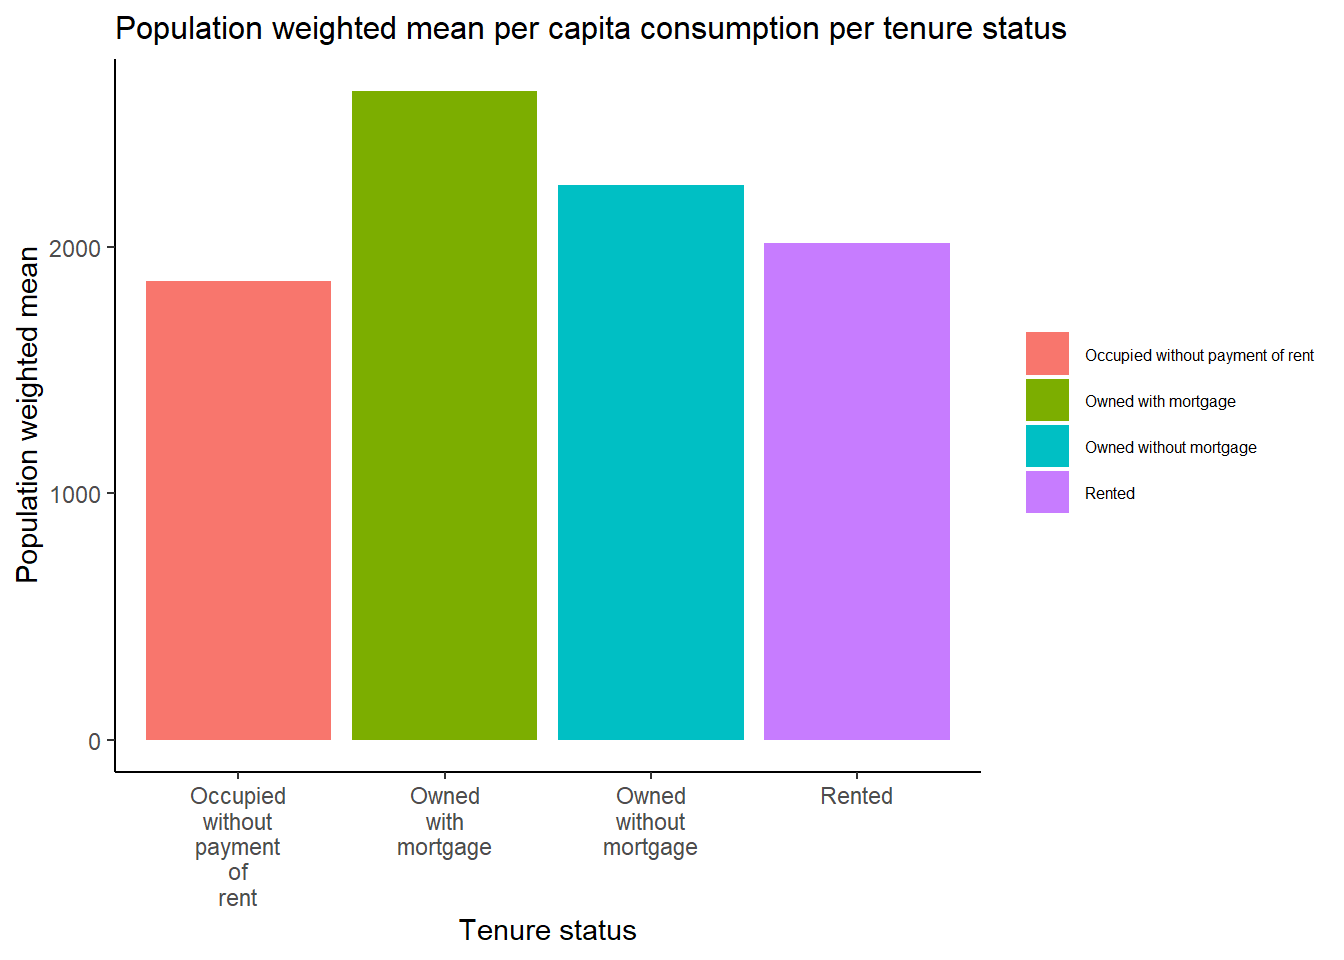
\includegraphics{02_Data_wrangling_homework_files/figure-latex/unnamed-chunk-22-1} \end{center}

\hypertarget{average-age-per-tenure-status}{%
\subsection{Average age per tenure
status}\label{average-age-per-tenure-status}}

We now want to calculate the average age per tenure status. For this we
need to calculate the average age per household member and join this
information to the household file. Do not bother with any population
weighting for this data wrangling step.

\hypertarget{calculate-the-average-age-per-household-using-the-person-file}{%
\subsubsection{Calculate the average age per household using the person
file}\label{calculate-the-average-age-per-household-using-the-person-file}}

The age variable is called ``age'' in the person object.

\hypertarget{join-the-average-age-per-household-to-the-household-file}{%
\subsubsection{Join the average age per household to the household
file}\label{join-the-average-age-per-household-to-the-household-file}}

The foreign key is called newid

\hypertarget{calculate-the-average-age-per-tenure-status}{%
\subsubsection{Calculate the average age per tenure
status}\label{calculate-the-average-age-per-tenure-status}}

Use the population weights for this step

\begin{Shaded}
\begin{Highlighting}[]
\NormalTok{person_clean <-}\StringTok{ }\NormalTok{person }\OperatorTok\StringTok{ }
\StringTok{  }\KeywordTok{group_by}\NormalTok{(newid) }\OperatorTok\StringTok{ }
\StringTok{  }\KeywordTok{mutate}\NormalTok{(}\DataTypeTok{avg_age =} \KeywordTok{mean}\NormalTok{(age)) }

\NormalTok{household_clean <-}\StringTok{ }\NormalTok{(}\KeywordTok{left_join}\NormalTok{(household_clean, person_clean, }\DataTypeTok{by=}\StringTok{"newid"}\NormalTok{)) }

\NormalTok{household_clean <-}\StringTok{ }\NormalTok{household_clean }\OperatorTok
\StringTok{    }\KeywordTok{select}\NormalTok{(newid, totexpcq, fam_size, cutenure, finlwt21, avg_age, pop_weighted_mean, exp_pc) }\OperatorTok\StringTok{ }
\StringTok{    }\KeywordTok{group_by}\NormalTok{(cutenure) }\OperatorTok\StringTok{ }
\StringTok{    }\KeywordTok{mutate}\NormalTok{(}\DataTypeTok{age_weighted_mean =} \KeywordTok{weighted.mean}\NormalTok{(avg_age,finlwt21))}
\KeywordTok{head}\NormalTok{(household_clean)}
\end{Highlighting}
\end{Shaded}

\begin{verbatim}
## # A tibble: 6 x 9
## # Groups:   cutenure [2]
##   newid totexpcq fam_size cutenure finlwt21 avg_age pop_weighted_me~ exp_pc
##   <chr>    <dbl>    <dbl> <chr>       <dbl>   <dbl>            <dbl>  <dbl>
## 1 0406~        0        3 Owned w~   36019.    42              2634.      0
## 2 0406~        0        3 Owned w~   36019.    42              2634.      0
## 3 0406~        0        3 Owned w~   36019.    42              2634.      0
## 4 0406~        0        2 Owned w~    2990.    52.5            2251.      0
## 5 0406~        0        2 Owned w~    2990.    52.5            2251.      0
## 6 0406~        0        4 Owned w~   25697.    22.5            2634.      0
## # ... with 1 more variable: age_weighted_mean <dbl>
\end{verbatim}

\hypertarget{create-a-bar-plot-that-compares-the-average-age-per-tenure-status}{%
\subsubsection{Create a bar plot that compares the average age per
tenure
status}\label{create-a-bar-plot-that-compares-the-average-age-per-tenure-status}}

Now use your result from above to create a bar plot using ggplot2. The
nicer it looks the better.

\begin{Shaded}
\begin{Highlighting}[]
\NormalTok{household_clean }\OperatorTok\StringTok{ }\NormalTok{ggplot }\OperatorTok{+}
\StringTok{  }\KeywordTok{geom_bar}\NormalTok{(}\DataTypeTok{mapping =} \KeywordTok{aes}\NormalTok{(}\DataTypeTok{x =}\NormalTok{ cutenure, }\DataTypeTok{y =}\NormalTok{ age_weighted_mean, }\DataTypeTok{fill =}\NormalTok{ cutenure), }\DataTypeTok{stat =} \StringTok{"summary"}\NormalTok{) }\OperatorTok{+}\StringTok{ }
\StringTok{  }\KeywordTok{labs}\NormalTok{(}\DataTypeTok{title =} \StringTok{"Average age per tenure status"}\NormalTok{, }\DataTypeTok{x =} \StringTok{"Tenure status"}\NormalTok{, }\DataTypeTok{y =} \StringTok{"Age weighted mean"}\NormalTok{) }\OperatorTok{+}\StringTok{ }
\StringTok{  }\KeywordTok{scale_x_discrete}\NormalTok{(}\DataTypeTok{breaks=}\KeywordTok{unique}\NormalTok{(household_clean}\OperatorTok{$}\NormalTok{cutenure), }\DataTypeTok{labels=}\KeywordTok{addline_format}\NormalTok{(}\KeywordTok{c}\NormalTok{(}\StringTok{"Owned with mortgage"}\NormalTok{,}\StringTok{"Owned without mortgage"}\NormalTok{,}\StringTok{"Rented"}\NormalTok{, }\StringTok{"Occupied without payment of rent"}\NormalTok{))) }\OperatorTok{+}
\StringTok{  }\KeywordTok{scale_fill_manual}\NormalTok{(}\DataTypeTok{values=}\KeywordTok{wes_palette}\NormalTok{(}\DataTypeTok{n=}\DecValTok{4}\NormalTok{, }\DataTypeTok{name=}\StringTok{"Darjeeling1"}\NormalTok{)) }\OperatorTok{+}
\StringTok{  }\NormalTok{theme_ds}
\end{Highlighting}
\end{Shaded}

\begin{verbatim}
## No summary function supplied, defaulting to `mean_se()`
\end{verbatim}

\begin{center}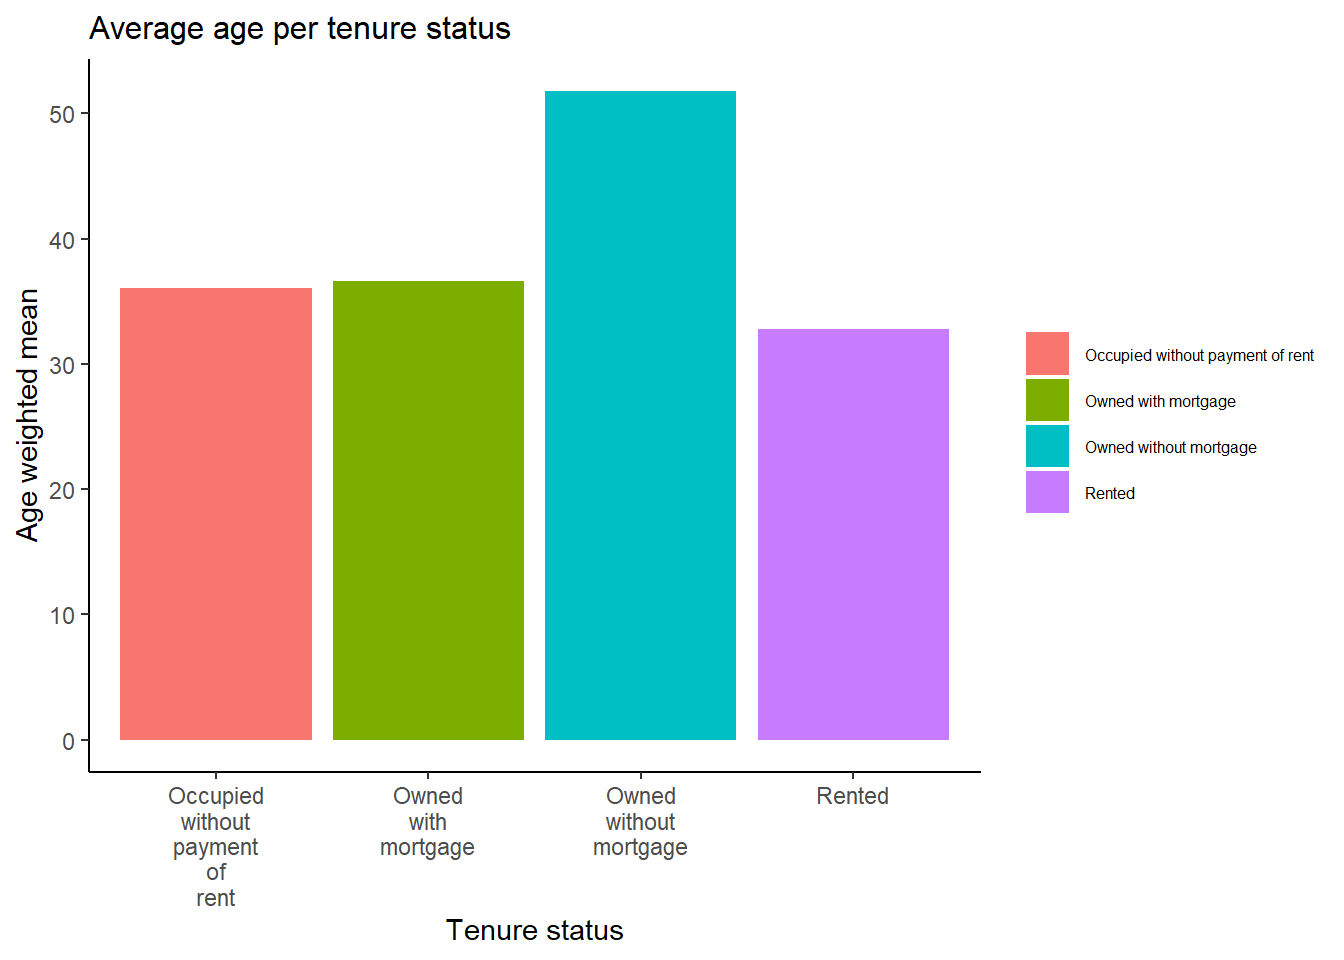
\includegraphics{02_Data_wrangling_homework_files/figure-latex/unnamed-chunk-24-1} \end{center}

\hypertarget{calculate-the-population-weighted-per-capita-consumption-per-average-household-age}{%
\subsubsection{Calculate the population weighted per capita consumption
per average household
age}\label{calculate-the-population-weighted-per-capita-consumption-per-average-household-age}}

\begin{itemize}
\tightlist
\item
  Round the average age per household to integer values
\item
  Use the split apply combine approach to calculate the population
  weighted per capita consumption per average household age
\item
  Arrange the results in an descending order
\item
  Display only the Top 10 results
\end{itemize}

\begin{Shaded}
\begin{Highlighting}[]
\NormalTok{household_clean <-}\StringTok{ }\NormalTok{household_clean }\OperatorTok\StringTok{ }
\StringTok{  }\KeywordTok{mutate}\NormalTok{(}\DataTypeTok{avg_age =} \KeywordTok{ceiling}\NormalTok{(avg_age)) }\OperatorTok\StringTok{ }
\StringTok{  }\KeywordTok{group_by}\NormalTok{(avg_age) }\OperatorTok\StringTok{ }
\StringTok{  }\KeywordTok{mutate}\NormalTok{(}\DataTypeTok{Pwccpaha =} \KeywordTok{weighted.mean}\NormalTok{(exp_pc,finlwt21)) }\OperatorTok
\StringTok{  }\KeywordTok{arrange}\NormalTok{(}\KeywordTok{desc}\NormalTok{(Pwccpaha)) }
 
\NormalTok{  household_clean }\OperatorTok\StringTok{ }\KeywordTok{head}\NormalTok{(}\DecValTok{10}\NormalTok{)}
\end{Highlighting}
\end{Shaded}

\begin{verbatim}
## # A tibble: 10 x 10
## # Groups:   avg_age [1]
##    newid totexpcq fam_size cutenure finlwt21 avg_age pop_weighted_me~ exp_pc
##    <chr>    <dbl>    <dbl> <chr>       <dbl>   <dbl>            <dbl>  <dbl>
##  1 0407~       0         1 Owned w~   19762.      83            2251.     0 
##  2 0410~    2046         1 Owned w~   24033.      83            2251.  2046 
##  3 0417~       0         1 Owned w~   35080.      83            2251.     0 
##  4 0418~       0         1 Rented     21949.      83            2018.     0 
##  5 0418~       0         1 Owned w~   20885.      83            2251.     0 
##  6 0418~    2441.        1 Owned w~   15392.      83            2251.  2441.
##  7 0419~    2714.        1 Rented     20208.      83            2018.  2714.
##  8 0419~   18393.        1 Owned w~   24239.      83            2251. 18393.
##  9 0421~       0         1 Owned w~   23291.      83            2634.     0 
## 10 0422~       0         1 Owned w~   19913.      83            2251.     0 
## # ... with 2 more variables: age_weighted_mean <dbl>, Pwccpaha <dbl>
\end{verbatim}

\hypertarget{create-an-appropriate-plot-to-display-the-data}{%
\subsubsection{Create an appropriate plot to display the
data}\label{create-an-appropriate-plot-to-display-the-data}}

\begin{itemize}
\tightlist
\item
  Use the results from above and plot the data
\item
  What do you conclude about the functional form of this relationship?
\item
  Run a regression to test your hypothesis
\end{itemize}

\begin{Shaded}
\begin{Highlighting}[]
\KeywordTok{ggplot}\NormalTok{(household_clean, }\KeywordTok{aes}\NormalTok{(}\DataTypeTok{x =}\NormalTok{ avg_age, }\DataTypeTok{y =}\NormalTok{ Pwccpaha, }\DataTypeTok{color =}\NormalTok{ cutenure)) }\OperatorTok{+}\StringTok{ }
\StringTok{  }\KeywordTok{geom_point}\NormalTok{() }\OperatorTok{+}
\StringTok{  }\KeywordTok{geom_smooth}\NormalTok{(}\DataTypeTok{method=}\StringTok{"loess"}\NormalTok{, }\DataTypeTok{se =}\NormalTok{ F, }\DataTypeTok{color=}\StringTok{"burlywood4"}\NormalTok{)  }\OperatorTok{+}
\StringTok{  }\KeywordTok{scale_fill_manual}\NormalTok{(}\DataTypeTok{values=}\KeywordTok{wes_palette}\NormalTok{(}\DataTypeTok{n=}\DecValTok{4}\NormalTok{, }\DataTypeTok{name=}\StringTok{"Darjeeling1"}\NormalTok{)) }\OperatorTok{+}
\StringTok{  }\NormalTok{theme_ds }\OperatorTok{+}
\StringTok{  }\KeywordTok{theme}\NormalTok{(}\DataTypeTok{legend.position =} \StringTok{"top"}\NormalTok{)}
\end{Highlighting}
\end{Shaded}

\begin{verbatim}
## `geom_smooth()` using formula 'y ~ x'
\end{verbatim}

\begin{center}\includegraphics{02_Data_wrangling_homework_files/figure-latex/unnamed-chunk-26-1} \end{center}

There seems to be a quadratic relatonship. This is why we decided to
include the squared average household age as a regressor.

\begin{Shaded}
\begin{Highlighting}[]
\NormalTok{household_clean <-}\StringTok{ }\NormalTok{household_clean }\OperatorTok\StringTok{ }
\StringTok{  }\KeywordTok{mutate}\NormalTok{(}\DataTypeTok{avg_age_2 =}\NormalTok{ avg_age}\OperatorTok{^}\DecValTok{2}\NormalTok{) }

\KeywordTok{library}\NormalTok{(jtools)}
\KeywordTok{library}\NormalTok{(kableExtra)}
\end{Highlighting}
\end{Shaded}

\begin{verbatim}
## 
## Attaching package: 'kableExtra'
\end{verbatim}

\begin{verbatim}
## The following object is masked from 'package:dplyr':
## 
##     group_rows
\end{verbatim}

\begin{Shaded}
\begin{Highlighting}[]
\NormalTok{lm2 <-}\StringTok{ }\KeywordTok{lm}\NormalTok{(}\DataTypeTok{data=}\NormalTok{household_clean, Pwccpaha }\OperatorTok{~}\StringTok{ }\NormalTok{avg_age }\OperatorTok{+}\StringTok{ }\NormalTok{avg_age_}\DecValTok{2}\NormalTok{)}
\KeywordTok{summ}\NormalTok{(lm2)}
\end{Highlighting}
\end{Shaded}

\begin{table}[!h]
\centering
\begin{tabular}{lr}
\toprule
\cellcolor{gray!6}{Observations} & \cellcolor{gray!6}{12520}\\
Dependent variable & Pwccpaha\\
\cellcolor{gray!6}{Type} & \cellcolor{gray!6}{OLS linear regression}\\
\bottomrule
\end{tabular}
\end{table} \begin{table}[!h]
\centering
\begin{tabular}{lr}
\toprule
\cellcolor{gray!6}{F(2,12517)} & \cellcolor{gray!6}{10811.08}\\
R² & 0.63\\
\cellcolor{gray!6}{Adj. R²} & \cellcolor{gray!6}{0.63}\\
\bottomrule
\end{tabular}
\end{table} \begin{table}[!h]
\centering
\begin{threeparttable}
\begin{tabular}{lrrrr}
\toprule
  & Est. & S.E. & t val. & p\\
\midrule
\cellcolor{gray!6}{(Intercept)} & \cellcolor{gray!6}{-74.92} & \cellcolor{gray!6}{18.00} & \cellcolor{gray!6}{-4.16} & \cellcolor{gray!6}{0.00}\\
avg\_age & 86.77 & 0.89 & 97.55 & 0.00\\
\cellcolor{gray!6}{avg\_age\_2} & \cellcolor{gray!6}{-0.70} & \cellcolor{gray!6}{0.01} & \cellcolor{gray!6}{-74.86} & \cellcolor{gray!6}{0.00}\\
\bottomrule
\end{tabular}
\begin{tablenotes}
\item Standard errors: OLS
\end{tablenotes}
\end{threeparttable}
\end{table}

As both the coefficient of the average household age and the squared
average household age are highly significant a quadratic form might be a
better starting point to model this relationship.

\begin{center}\rule{0.5\linewidth}{0.5pt}\end{center}

\end{document}
